
If you have ever used GNU Make, you will have already seen the concept of a target. Essentially, it's a recipe that a buildsystem uses to compile a list of files into another file. It can be a .cpp implementation file compiled into an .o object file, a group of .o files packaged into an .a static library, and many other combinations.

CMake, however, allows you to save time and skip the intermediate steps of those recipes; it works on a higher level of abstraction. It understands how to build an executable directly from source files. So, you don't need to write an explicit recipe to compile any object files. All that's required is an add\_executable() command with the name of the executable target and a list of the files that are to be its elements:

\begin{lstlisting}[style=styleCMake]
add_executable(app1 a.cpp b.cpp c.cpp)
\end{lstlisting}

We already used this command in previous chapters and we already know how executable targets are used in practice – during the generation step, CMake will create a buildsystem and fill it with recipes to compile each of the source files and link them together into a single binary executable.

In CMake, we can create a target using one of three commands:

\begin{itemize}
\item 
add\_executable()

\item 
add\_library()

\item 
add\_custom\_target()
\end{itemize}

The first two are pretty self-explanatory; we briefly used them already in previous chapters to build executables and libraries (and we'll discuss them in depth in Chapter 5, Compiling C++ Sources with CMake). But what are those custom targets?

They allow you to specify your own command line that will be executed without checking whether the produced output is up to date, for example:

\begin{itemize}
\item 
Calculate the checksums of other binaries.

\item 
Run the code-sanitizer and collect the results.

\item 
Send a compilation report to the data processing pipeline.
\end{itemize}

Here's the full signature of the add\_custom\_target() command:

\begin{lstlisting}[style=styleCMake]
add_custom_target(Name [ALL] [command1 [args1...]]
				[COMMAND command2 [args2...] ...]
				[DEPENDS depend depend depend ... ]
				[BYPRODUCTS [files...]]
				[WORKING_DIRECTORY dir]
				[COMMENT comment]
				[JOB_POOL job_pool]
				[VERBATIM] [USES_TERMINAL]
				[COMMAND_EXPAND_LISTS]
				[SOURCES src1 [src2...]])
\end{lstlisting}

We won't discuss every option here, as we want to quickly move on to other targets, but let's just say that custom targets don't necessarily have to produce tangible artifacts in the form of files.

One good use case for custom targets might be the need to remove specific files on every build – for example, to make sure that code-coverage reports don't contain stale data. All we need to do is define a custom target like so:

\begin{lstlisting}[style=styleCMake]
add_custom_target(clean_stale_coverage_files
		COMMAND find . -name "*.gcda" -type f -delete)
\end{lstlisting}

The preceding command will search for all files with a .gcda extension and remove them. There is one catch though; unlike executable and library targets, custom targets won't be built until they are added to a dependency graph. Let's find out what that is.

\subsubsubsection{4.2.1\hspace{0.2cm}Dependency graph}

Mature applications are often built from many components, and I don't mean external dependencies here. Specifically, I'm talking about internal libraries. Adding them to the project is useful from a structural perspective, as related things are packaged together in a single logical entity. And they can be linked with other targets – another library or an executable. This is especially convenient when multiple targets are using the same library. Take a look at Figure 4.1, which describes an exemplary dependency graph:

\begin{center}
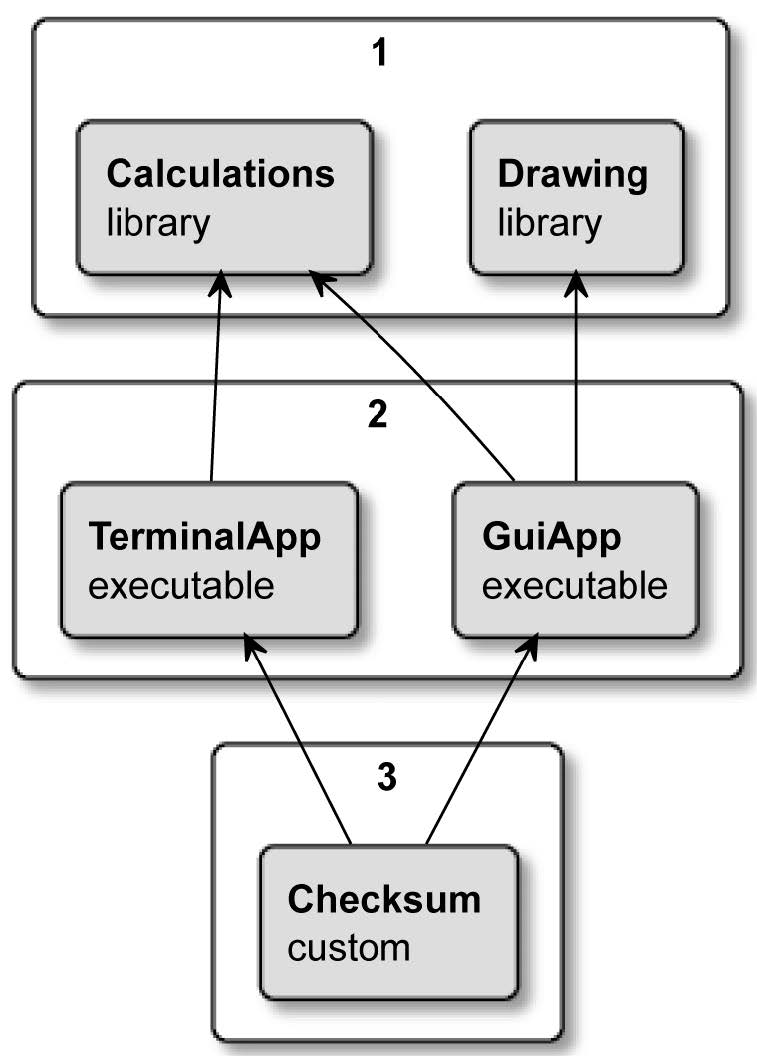
\includegraphics[width=0.5\textwidth]{content/2/chapter4/images/1.jpg}\\
Figure 4.1 – Order of building dependencies in the BankApp project
\end{center}

In this project, we have two libraries, two executables, and a custom target. Our use case here is to provide a banking application with a nice GUI for users (GuiApp), and a command-line version to be used as part of an automated script (TerminalApp). Both executables are depending on the same Calculations library, but only one of them needs the Drawing library. To guarantee that our app wasn't modified when it was downloaded from the internet by an end user, we'll calculate a checksum, store it in a file, and distribute it through separate secure channels. CMake is pretty flexible when it comes to writing list files for such a solution:

\begin{lstlisting}[style=styleCMake]
# chapter04/01-targets/CMakeLists.txt

cmake_minimum_required(VERSION 3.19.2)
project(BankApp CXX)

add_executable(terminal_app terminal_app.cpp)
add_executable(gui_app gui_app.cpp)

target_link_libraries(terminal_app calculations)
target_link_libraries(gui_app calculations drawing)

add_library(calculations calculations.cpp)
add_library(drawing drawing.cpp)

add_custom_target(checksum ALL
	COMMAND sh -c "cksum terminal_app>terminal.ck"
	COMMAND sh -c "cksum gui_app>gui.ck"
	BYPRODUCTS terminal.ck gui.ck
	COMMENT "Checking the sums..."
)
\end{lstlisting}

We connect our libraries with executables by using the target\_link\_libraries() command. Without it, the compilation for executables would fail because of undefined symbols. Have you noticed that we invoked this command before actually declaring any of the libraries? When CMake configures the project, it collects the information about targets and their properties – their names, dependencies, source files, and other details.

After parsing all the files, CMake will attempt to build a dependency graph. And like with all valid dependency graphs, they're directional acyclic graphs. This means that there is a clear direction of which target depends on which, and such dependencies cannot form cycles.

When we execute cmake in build mode, the generated buildsystem will check what top-level targets we have defined and recursively build their dependencies. Let's consider our example from Figure 4.1:

\begin{enumerate}
\item 
Start from the top, and build both libraries in group 1.

\item 
When the Calculations and Drawing libraries are complete, build group 2 – GuiApp and TerminalApp.

\item 
Build a checksum target; run specified command lines to generate checksums (cksum is a Unix checksum tool).
\end{enumerate}

There's a slight issue though – the preceding solution doesn't guarantee that a checksum target will be built after executables. CMake doesn't know that a checksum depends on the executable binaries being present, so it's free to start building it first. To resolve this problem, we can put the add\_dependencies() command at the end of the file:

\begin{lstlisting}[style=styleCMake]
add_dependencies(checksum terminal_app gui_app)
\end{lstlisting}

This will ensure that CMake understands the relation between the Checksum target and the executables.

That's great, but what's the difference between target\_link\_libraries() and add\_dependencies()? The first is intended to be used with actual libraries and allows you to control property propagation. The second is meant to be used only with top-level targets to set their build order.

As projects grow in complexity, the dependency tree gets harder to understand. How can we simplify this process?

\subsubsubsection{4.2.2\hspace{0.2cm}Visualizing dependencies}

Even small projects can be difficult to reason about and share with other developers. The easiest way to do so is through a nice diagram. After all, a picture is worth a thousand words. We can do the work and draw a diagram ourselves, just like I did in Figure 4.1. But this is tedious and would require constant updates. Luckily, CMake has a great module to generate dependency graphs in the dot/graphviz format. And it supports both internal and external dependencies!

To use it, we can simply execute this command:

\begin{tcblisting}{commandshell={}}
cmake --graphviz=test.dot .
\end{tcblisting}

The module will produce a text file that we can import to the Graphviz visualization software, which can render an image or produce a PDF or SVG file that can be stored as part of the software documentation. Everybody loves great documentation, but hardly anyone likes to create it – now, you don't need to!

If you're in a rush, you can even run Graphviz straight from your browser at this address:

\url{https://dreampuf.github.io/GraphvizOnline/}

\begin{tcolorbox}[colback=blue!5!white,colframe=blue!75!black,title=Important Note]
Custom targets are not visible by default and we need to create a special configuration file, CMakeGraphVizOptions.cmake, that will allow us to customize the graph. One handy customization command is set(GRAPHVIZ\_CUSTOM\_TARGETS TRUE); add it to the special configuration file to enable reporting custom targets in your graph. You can find more options in the documentation for the module.
\end{tcolorbox}

All you need to do is copy and paste the contents of the test.dot file into the window on the left and your project will be visualized. Quite convenient, isn't it?

\begin{center}
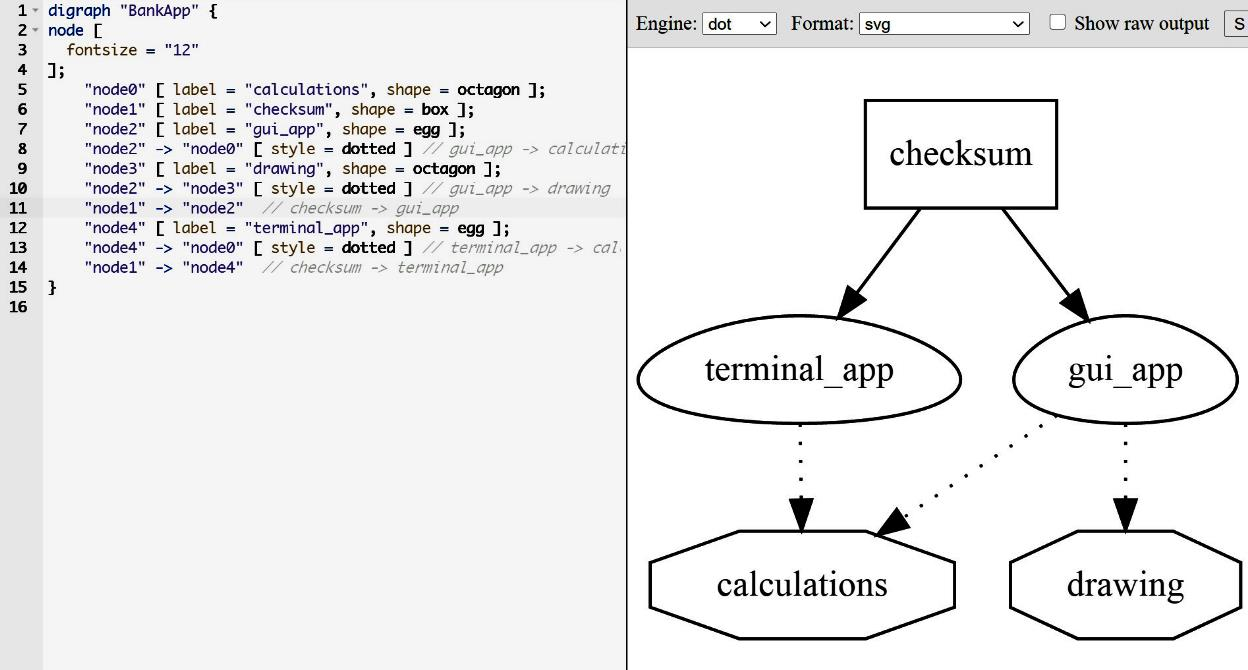
\includegraphics[width=0.8\textwidth]{content/2/chapter4/images/2.jpg}\\
Figure 4.2 – A visualization of the BankApp example in Graphviz
\end{center}

I have removed the automatically generated legend section from the preceding figure for clarity.

Using this method, we can quickly see all the explicitly defined targets. Now that we have this global perspective, let's do a deep dive and see how to configure them.
 
\subsubsubsection{4.2.3\hspace{0.2cm}Target properties}

Targets have properties that work in a similar way to fields of C++ objects. We can modify some of these properties and others are read-only. CMake defines a large list of "known properties" (see the Further reading section) that are available depending on the type of the target (executable, library, or custom). You can also add your own properties if you like. Use the following commands to manipulate the properties of a target:

\begin{lstlisting}[style=styleCMake]
get_target_property(<var> <target> <property-name>)
set_target_properties(<target1> <target2> ...
						PROPERTIES <prop1-name> <value1>
						<prop2-name> <value2> ...)
\end{lstlisting}

To print a target property on screen, we first need to store it in the <var> variable and then message() it to the user; we have to read them one by one. On the other hand, setting properties on a target allows us to specify multiple properties at the same time, on multiple targets.

The concept of properties isn't unique to targets; CMake supports setting properties of other scopes as well: GLOBAL, DIRECTORY, SOURCE, INSTALL, TEST, and CACHE.

To manipulate all kinds of properties, there are general get\_property() and set\_property() commands. You can use these low-level commands to do exactly what the set\_target\_properties() command does, just with a bit more work:

\begin{lstlisting}[style=styleCMake]
set_property(TARGET <target> PROPERTY <name> <value>)
\end{lstlisting}

Generally, it's better to use as many high-level commands as you can. CMake offers more of these, even narrower in their scope, such as setting specific properties on a target. For example, add\_dependencies(<target> <dep>) is appending dependencies to the MANUALLY\_ADDED\_DEPENDENCIES target property. In this case, we can query it with get\_target\_property() exactly as with any other property. However, we can't use set\_target\_property() to change it (it's read-only), as CMake insists on using the add\_dependencies() command to restrict operations to appending only.

We'll introduce more property setting commands when we discuss compiling and linking in upcoming chapters. Meanwhile, let's focus on how the properties of one target can transition to another.

\subsubsubsection{4.2.4\hspace{0.2cm}What are transitive usage requirements?}

Let's just agree that naming is hard, and sometimes one ends up with a result that's hard to understand. "Transitive usage requirements" is, unfortunately, one of those cryptic titles that you will encounter in the online CMake documents. Let's untangle this strange name and perhaps propose a term easier to understand.

I'll start by clarifying the middle bit of this puzzle. As we previously discussed, one target may depend on another. CMake documentation sometimes refers to such dependency as usage, as in one target uses another. This was straightforward, so on to the next one.

There will be cases when such a used target has specific requirements that a using target has to meet: link some libraries, include a directory, or require specific compile features. All of these are in fact requirements, so documentation is correct in a sense. The issue is that they aren't called requirements in any other context in the documentation. When you specify the same requirements for a single target, you set properties or dependencies. Therefore, the last part of the name should perhaps be simply "properties."

The last part is –transitive. This one I believe is correct (maybe a bit too smart). CMake appends some properties/requirements of used targets to properties of targets using them. You can say that some properties can transition (or simply propagate) across targets implicitly, so it's easier to express dependencies.

Simplifying this whole concept, I see it as propagated properties between the source target (targets that gets used) and destination targets (targets that use other targets).

Let's look at a concrete example to understand why it's there and how it works:

\begin{lstlisting}[style=styleCMake]
target_compile_definitions(<source> <INTERFACE|PUBLIC|PRIVATE> 
	[items1...])
\end{lstlisting}

This target command will populate the COMPILE\_DEFINITIONS property of a <source> target. Compile definitions are simply -Dname=definition flags passed to the compiler that configure the C++ preprocessor definitions (we'll get to that in Chapter 5, Compiling C++ Sources with CMake). The interesting part here is the second argument. We need to specify one of three values, INTERFACE, PUBLIC, or PRIVATE, to control which targets the property should be passed to. Now, don't confuse these with C++ access specifiers – this is something else.

Propagation keywords work like this:

\begin{itemize}
\item 
PRIVATE sets the property of the source target.

\item 
INTERFACE sets the property of the destination targets.

\item 
PUBLIC sets the property of the source and destination targets.
\end{itemize}

When a property is not to be transitioned to any destination targets, set it to PRIVATE.
When such a transition is needed, go with PUBLIC. If you're in a situation where the source target doesn't use the property in its implementation (.cpp files) and only in headers, and these are passed to the consumer targets, INTERFACE is the answer.

How does this work under the hood? To manage those properties, CMake provides a few commands such as the aforementioned target\_compile\_definitions(). When you specify a PRIVATE or PUBLIC keyword, CMake will store provided values in the property of the target matching the command – in this case, COMPILE\_DEFINITIONS. Additionally, if a keyword was INTERFACE or PUBLIC, it will store the value in property with an INTERFACE\_ prefix – INTERFACE\_COMPILE\_DEFINITIONS. During the configuration stage, CMake will read the interface properties of source targets and append their contents to destination targets. There you have it – propagated properties, or transitive usage requirements – as CMake calls them.

In CMake 3.20, there are 12 such properties managed with appropriate commands such as target\_link\_options() or directly with the set\_target\_properties() command:

\begin{itemize}
\item 
AUTOUIC\_OPTIONS

\item 
COMPILE\_DEFINITIONS

\item 
COMPILE\_FEATURES

\item 
COMPILE\_OPTIONS

\item 
INCLUDE\_DIRECTORIES

\item 
LINK\_DEPENDS

\item 
LINK\_DIRECTORIES

\item 
LINK\_LIBRARIES

\item 
LINK\_OPTIONS

\item 
POSITION\_INDEPENDENT\_CODE

\item 
PRECOMPILE\_HEADERS

\item 
SOURCES
\end{itemize}

We'll discuss most of these options in the following pages, but remember that all of these options are, of course, described in the CMake manual. Find them on their own page under a URL in this format (replace <PROPERTY> with a property that interests you): 

\url{https://cmake.org/cmake/help/latest/prop_tgt/<PROPERTY>.html}

The next question that comes to mind is how far this propagation goes. Are the properties set just on the first destination target, or are they sent to the very top of the dependency graph? Actually, you get to decide.

To create a dependency between targets, we use the target\_link\_libraries() command. The full signature of this command requires a propagation keyword:

\begin{lstlisting}[style=styleCMake]
target_link_libraries(<target>
					<PRIVATE|PUBLIC|INTERFACE> <item>...
					[<PRIVATE|PUBLIC|INTERFACE> <item>...]...)
\end{lstlisting}

As you can see, this signature also specifies a propagation keyword, but this one controls where properties from the source target get stored in the destination target. Figure 4.3 shows what happens to a propagated property during the generation stage (after the configuration stage is completed):

\begin{center}
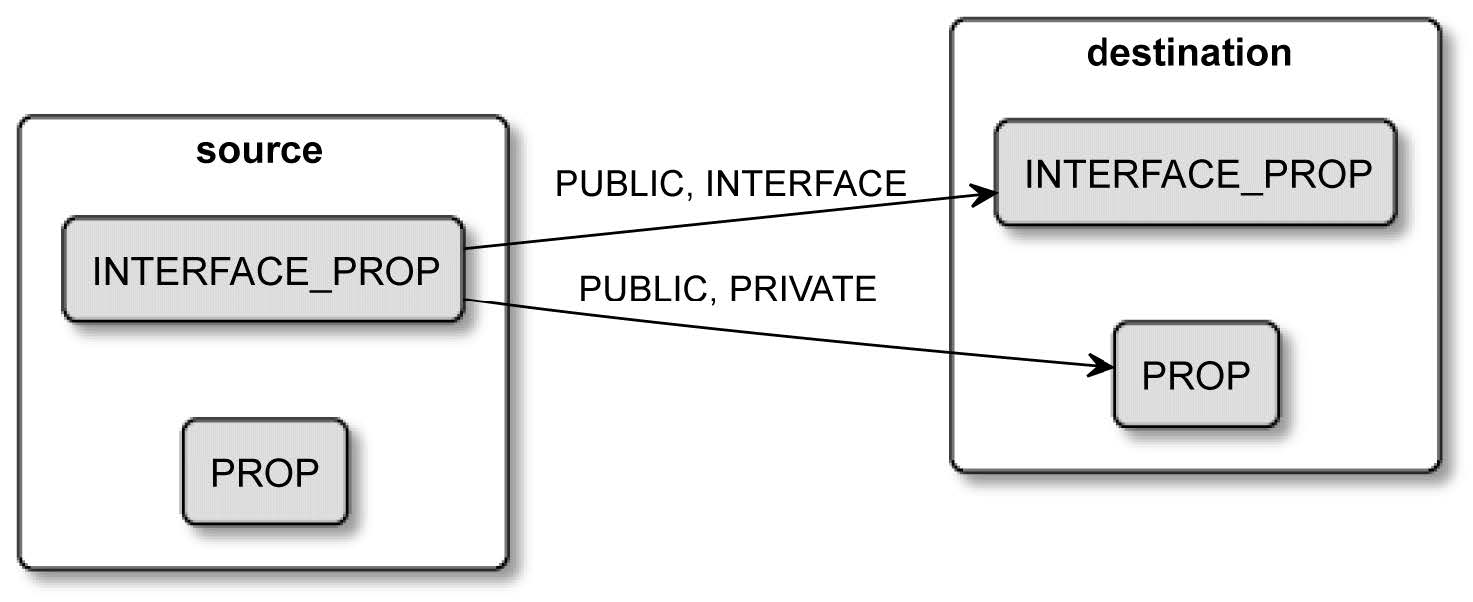
\includegraphics[width=0.8\textwidth]{content/2/chapter4/images/3.jpg}\\
Figure 4.3 – How properties are propagated to destination targets
\end{center}

Propagation keywords work like this:

\begin{itemize}
\item 
PRIVATE appends the source value to the private property of the destination.

\item 
INTERFACE appends the source value to the interface property of the destination.

\item 
PUBLIC appends to both properties of the destination.
\end{itemize}

As we discussed before, interface properties are only used to propagate the properties further down the chain, and the destination target won't use them in its build process.

The basic target\_link\_libraries(<target> <item>...) command that we used before implicitly specifies the PUBLIC keyword.

If you correctly set propagation keywords for your source targets, properties will be automatically placed on destination targets for you – unless there's a conflict…

\subsubsubsection{4.2.5\hspace{0.2cm}Dealing with conflicting propagated properties}

When one target depends on multiple other targets, there may be a situation where propagated properties are in outright conflict with each other. Say that one used target specifies the POSITION\_INDEPENDENT\_CODE property as true and the other as false. CMake understands this as a conflict and will print an error similar to this:

\begin{tcblisting}{commandshell={}}
CMake Error: The INTERFACE_POSITION_INDEPENDENT_CODE property
of "source_target2" does not agree with the value of POSITION_
INDEPENDENT_CODE already determined for "destination_target".
\end{tcblisting}

It is useful to receive such a message, as we explicitly know that we introduced this conflict and we need to resolve it. CMake has its own properties that have to "agree" between source and destination targets.

On rare occasions, this may become important – for example, if you're building software using the same library in multiple targets that are then linked to a single executable. If these source targets are using different versions of the same library, you may run into problems.

To make sure that we're only using the same specific version, we can create a custom interface property, INTERFACE\_LIB\_VERSION, and store the version there. This is not enough to solve the problem, as CMake won't propagate custom properties by default. We have to explicitly add a custom property to a list of "compatible" properties.

Each target has four such lists:

\begin{itemize}
\item 
COMPATIBLE\_INTERFACE\_BOOL

\item 
COMPATIBLE\_INTERFACE\_STRING

\item 
COMPATIBLE\_INTERFACE\_NUMBER\_MAX

\item 
COMPATIBLE\_INTERFACE\_NUMBER\_MIN
\end{itemize}

Appending your property to one of them will trigger propagation and compatibility checks. The BOOL list will check whether all properties propagated to the destination target evaluate to the same Boolean value. Analogically, STRING will evaluate to a string. NUMBER\_MAX and NUMBER\_MIN are a bit different – propagated values don't have to match, but the destination target will just receive the highest or the lowest value instead.

This example will help us to understand how to apply this in practice:

\begin{lstlisting}[style=styleCMake]
# chapter04/02-propagated/CMakeLists.txt

cmake_minimum_required(VERSION 3.20.0)
project(PropagatedProperties CXX)

add_library(source1 empty.cpp)
set_property(TARGET source1 PROPERTY INTERFACE_LIB_VERSION
	4)
set_property(TARGET source1 APPEND PROPERTY
	COMPATIBLE_INTERFACE_STRING LIB_VERSION
)
add_library(source2 empty.cpp)

set_property(TARGET source2 PROPERTY INTERFACE_LIB_VERSION
	4)
add_library(destination empty.cpp)
target_link_libraries(destination source1 source2)
\end{lstlisting}

We create three targets here; for simplicity, all are using the same empty source file. On both of the source targets, we specify our custom property with the INTERFACE\_ prefix. And we set them to the same matching library version. Both of the source targets are linked to the destination target. Finally, we specify a STRING compatibility requirement as a property for source1 (we don't add the INTERFACE\_ prefix here).

CMake will propagate this custom property to the destination target and check whether the version of all the source targets is an exact match (the compatibility property can be set on just one target).

Now that we understand what targets are, let's take a look at other things that look like targets, smell like targets, and sometimes act like targets but, as it turns out, aren't the real deal.

\subsubsubsection{4.2.6\hspace{0.2cm}Meet the pseudo targets}

The concept of a target is so useful that it would be great if some of its behaviors could be borrowed for other things too. This is, specifically, things that do not represent outputs of the buildsystem but rather inputs – external dependencies, aliases, and so on. These are the pseudo targets, or targets that don't make it to the generated buildsystem.

\hspace*{\fill} \\ %插入空行
\noindent
\textbf{Imported targets}

If you skimmed the table of contents, you know that we'll be talking about how CMake manages external dependencies – other projects, libraries, and so on. IMPORTED targets are essentially products of this process. CMake can define them as a result of the find\_ package() command.

You can adjust the target properties of such a target: compile definitions, compile options, include directories, and so on – and they will even support transitive usage requirements. However, you should treat them as immutable; don't change their sources or dependencies.

The scope of the definition of an IMPORTED target can be global or local to the directory where it was defined (visible in subdirectories but not in parent directories).

\hspace*{\fill} \\ %插入空行
\noindent
\textbf{Alias targets}

Alias targets do exactly what you expect – they create another reference to a target under a different name. You can create alias targets for executables and libraries with the following commands:

\begin{lstlisting}[style=styleCMake]
add_executable(<name> ALIAS <target>)
add_library(<name> ALIAS <target>)
\end{lstlisting}

Properties of alias targets are read-only, and you cannot install or export aliases (they aren't visible in the generated buildsystem).

So, what is the reason to have aliases at all? They come in handy in scenarios where some part of a project (such as a subdirectory) requires a target with a specific name, and the actual implementation may be available under different names depending on circumstances. For example, you may wish to build a library shipped with your solution or import it based on a user's choice.

\hspace*{\fill} \\ %插入空行
\noindent
\textbf{Interface libraries}

This is an interesting construct – a library that doesn't compile anything but instead serves as a utility target. Its whole concept is built around propagated properties (transitive usage requirements).

Interface libraries have two primary uses – to represent header-only libraries and to bundle a bunch of propagated properties into a single logical unit.

Header-only libraries are fairly easy to create with add\_library(INTERFACE):

\begin{lstlisting}[style=styleCMake]
add_library(Eigen INTERFACE
	src/eigen.h src/vector.h src/matrix.h
)
target_include_directories(Eigen INTERFACE
	$<BUILD_INTERFACE:${CMAKE_CURRENT_SOURCE_DIR}/src>
	$<INSTALL_INTERFACE:include/Eigen>
)
\end{lstlisting}

In the preceding snippet, we created an Eigen interface library with three headers. Next, with generator expressions (explained in the last section of this chapter), we set its include directories to be \$\{CMAKE\_CURRENT\_SOURCE\_DIR\}/src when a target is exported and include/Eigen when it's installed (which will also be explained at the end of this chapter).

To use such a library, we just have to link it:

\begin{lstlisting}[style=styleCMake]
target_link_libraries(executable Eigen)
\end{lstlisting}

No actual linking occurs here, but CMake will understand this command as a request to propagate all the INTERFACE properties to the executable target.

The second use case leverages exactly the same mechanism but for a different purpose – it creates a logical target that can be a placeholder for propagated properties. We can then use this target as a dependency for other targets and set properties in a clean, convenient way. Here's an example:

\begin{lstlisting}[style=styleCMake]
add_library(warning_props INTERFACE)
target_compile_options(warning_props INTERFACE
	-Wall -Wextra -Wpedantic
)
target_link_libraries(executable warning_props)
\end{lstlisting}

The add\_library(INTERFACE) command creates a logical warning\_props target that is used to set compile options specified in the second command on the executable target. I recommend using these INTERFACE targets, as they improve the readability and reusability of your code. Think of it as refactoring a bunch of magic values to a wellnamed variable. I also suggest using the \_props suffix to easily differentiate interface libraries from the regular ones.

Are pseudo targets exhausting the concept of the target? Of course not! That would simply be too easy. We still need to understand how these targets translate to produced buildsystems.

\subsubsubsection{4.2.7\hspace{0.2cm}Build targets}

Target is a bit of a loaded word. It means different things in the context of a project and the context of generated buildsystems. When CMake generates a buildsystem, it "compiles" list files from CMake language to the language of a chosen build tool; perhaps it creates a Makefile for GNU Make. Such Makefiles have their own targets – some of them are direct conversions of list file targets, and others are created implicitly.

One such buildsystem target is ALL, which CMake generates by default to contain all top-level list file targets, such as executables and libraries (not necessarily custom targets). ALL is built when we run cmake -{}-build <build tree> without choosing a concrete target. As you might remember from the first chapter, you can choose one by adding the -{}-target <name> parameter to the preceding command.

Some executables or libraries might not be needed in every build, but we'd like to keep them as part of the project for those rare occasions when they come in useful. To optimize our default build, we can exclude them from the ALL target like so:

\begin{lstlisting}[style=styleCMake]
add_executable(<name> EXCLUDE_FROM_ALL [<source>...])
add_library(<name> EXCLUDE_FROM_ALL [<source>...])
\end{lstlisting}

Custom targets work the other way around – by default, they're excluded from the ALL target unless you explicitly define them with an ALL keyword, as we did in the BankApp example.

Another implicitly defined build target is clean, which simply removes produced artifacts from the build tree. We use it to get rid of all old files and build everything from scratch. It's important though to understand that it don't just simply delete everything in the build directory. This means that for clean to work correctly, you need to manually specify any files that your custom targets might create as BYPRODUCTS (see the BankApp example).

There's also an interesting non-target mechanism to create custom artifacts that can be used in all actual targets – custom commands.

